\section{Trabajo Teórico}

\subsection{\textit{Derivación del sistema de control}}

En primer lugar para estudiar el sistema MIMO de la figura \ref{fig:circuito}, se aplicó 
la ley de voltaje de Kirchhoff en el nodo que esta arriba del condensador C$_{\text{L}}$, 
obteniéndose la siguiente ecuación,

\begin{equation}
    i_{\text{FC}} + i_{\text{B}} = i_{\text{L}} + i_{\text{CL}}
\end{equation}

Luego utilizando ley de Ohm se puede llegar a la expresión:

\begin{equation}
    i_{\text{FC}} + i_{\text{B}} = \frac{v_{\text{CL}}}{R_{\text{L}}} + C_{L}\frac{dv_{\text{CL}}}{dt}
\end{equation}

Que en el dominio de la frecuencia equivale a:

\begin{equation}
    I_{\text{FC}} + I_{\text{B}} = \frac{V_{\text{CL}}}{R_{\text{L}}} + sC_{L}V_{\text{CL}}
\end{equation}

Y si despejamos la variable a controlar, V$_{\text{CL}}$, se llega a

\begin{equation}
    V_{\text{CL}} = \frac{R_{\text{L}}}{1+sC_{\text{L}}R_{\text{L}}}(I_{\text{FC}}+I_{\text{B}})
    \label{eq:lazoext}
\end{equation}

Por tanto notar que por (\ref{eq:lazoext}), es posible controlar el voltaje de la carga con las corrientes I$_{\text{FC}}$ e I$_{\text{B}}$.

Ahora bien, dado que los sistemas operan en velocidades sumamente diferentes, 140 rad/s vs 4 rad/s,
se estudiarán por separado. La planta de las celdas de combustible (Fuel Cell) queda de la siguiente
forma.

\begin{center}
\begin{tikzpicture}
	% Paths, nodes and wires:
	\draw (0, 3) to[battery, l={$V_{FC}$}, label distance=0.02cm] (0, 0);
	\draw (0, 3) to[american inductor, l={$L_{FC}$}, label distance=0.02cm] (3, 3);
	\draw (3, 3) to[american resistor, l={$R_{FC}$}, label distance=0.02cm] (6, 3);
	\draw (6, 0) to[capacitor, l={$C_L$}, label distance=0.02cm, v=$V_{CL}$] (6, 3);
	\draw (0, 0) -- (6, 0);
	\draw node[vcc, rotate=-90] (N1) at (2.75, 3) {} node[anchor=south east] at ([xshift=0cm, yshift=-0.62cm]N1.text){$I_{FC}$};
\end{tikzpicture}
\end{center}

Y la planta de las baterías,

\begin{center}
\begin{tikzpicture}
	% Paths, nodes and wires:
	\draw node[vcc, rotate=-90, yscale=-1] (N1) at (3.25, 3) {} node[anchor=south east] at ([xshift=0.62cm, yshift=-0.62cm]N1.text){$I_{B}$};
	\node[shape=rectangle, draw, line width=1pt, inner sep=0, minimum width=-0.035cm, minimum height=-0.035cm] at (7, 1.5){};
	\draw (3, 3) to[american inductor, l_={$L_{B}$}, label distance=0.02cm, mirror] (0, 3);
	\draw (6, 3) to[american resistor, l_={$R_{B}$}, label distance=0.02cm, mirror] (3, 3);
	\draw (6, 3) to[battery, l={$V_{B}$}, label distance=0.02cm] (6, -0);
	\draw (0, 0) to[capacitor,v=$V_{CL}$, l={$C_{L}$}, label distance=0.02cm] (0, 3);
	\draw (0, 0) -- (6, 0);
\end{tikzpicture}
\end{center}

Luego las ecuaciones que rigen ambos circuitos usando LVK son (\ref{ecuacion batería}) para la batería y (\ref{ecuacion Fuel Cell}) para la fuel cell,

\begin{equation}\label{ecuacion batería}
    V_{\text{B}} - I_{\text{B}}(R_{\text{B}} + sL_{\text{B}}) - V_{\text{CL}} = 0
\end{equation}
\begin{equation}\label{ecuacion Fuel Cell}
    V_{\text{FC}} - I_{\text{FC}}(R_{\text{FC}} + sL_{\text{FC}}) - V_{\text{CL}} = 0
\end{equation}

Manipulando las ecuaciones se pueden despejar las corrientes,

\begin{equation}
    I_{\text{B}} = \frac{V_{\text{B}}- V_{\text{CL}}}{(R_{\text{B}} + sL_{\text{B}})} 
\end{equation}
\begin{equation}
    I_{\text{FC}} = \frac{V_{\text{FC}}- V_{\text{CL}}}{(R_{\text{FC}} + sL_{\text{FC}})} 
\end{equation}

Recordar que V$_{\text{B}}$ y V$_{\text{FC}}$ son las entradas del sistema, y por tanto es posible controlar las corrientes mencionadas con anterioridad.

Además la corriente de carga se obtiene por ley de Ohm,

\begin{equation}
    I_{\text{L}} = \frac{V_{\text{CL}}}{R_{\text{L}}}
\end{equation}

Entonces, juntando todo se obtiene que el sistema MIMO queda descrito por las siguientes funciones de transferencia,

\begin{equation}\label{Funcion de transferencia batería interno}
    \frac{I_{\text{B}}}{V_{\text{B}}- V_{\text{CL}}}=\frac{1}{R_{\text{B}} + sL_{\text{B}}} 
\end{equation}

\begin{equation}\label{Funcion de transferencia fuel cell}
    \frac{I_{\text{FC}}}{V_{\text{FC}}- V_{\text{CL}}}=\frac{1}{R_{\text{FC}} +sL_{\text{FC}}} 
\end{equation}

\begin{equation}\label{Funcion de transferencia batería externo}
    \frac{V_{\text{CL}}}{I_{\text{FC}}+I_{\text{B}}}=\frac{R_{\text{L}}}{1+sC_{\text{L}}R_{\text{L}}}
\end{equation}

%Por tanto el diagrama de bloques teniendo en consideración que se deben tener tres controladores, uno para el lazo de celdas de combustibles, y otros dos para el lazo interno y externo de las baterías, queda entonces de la siguiente forma,

% \begin{figure}
%     \centering
%     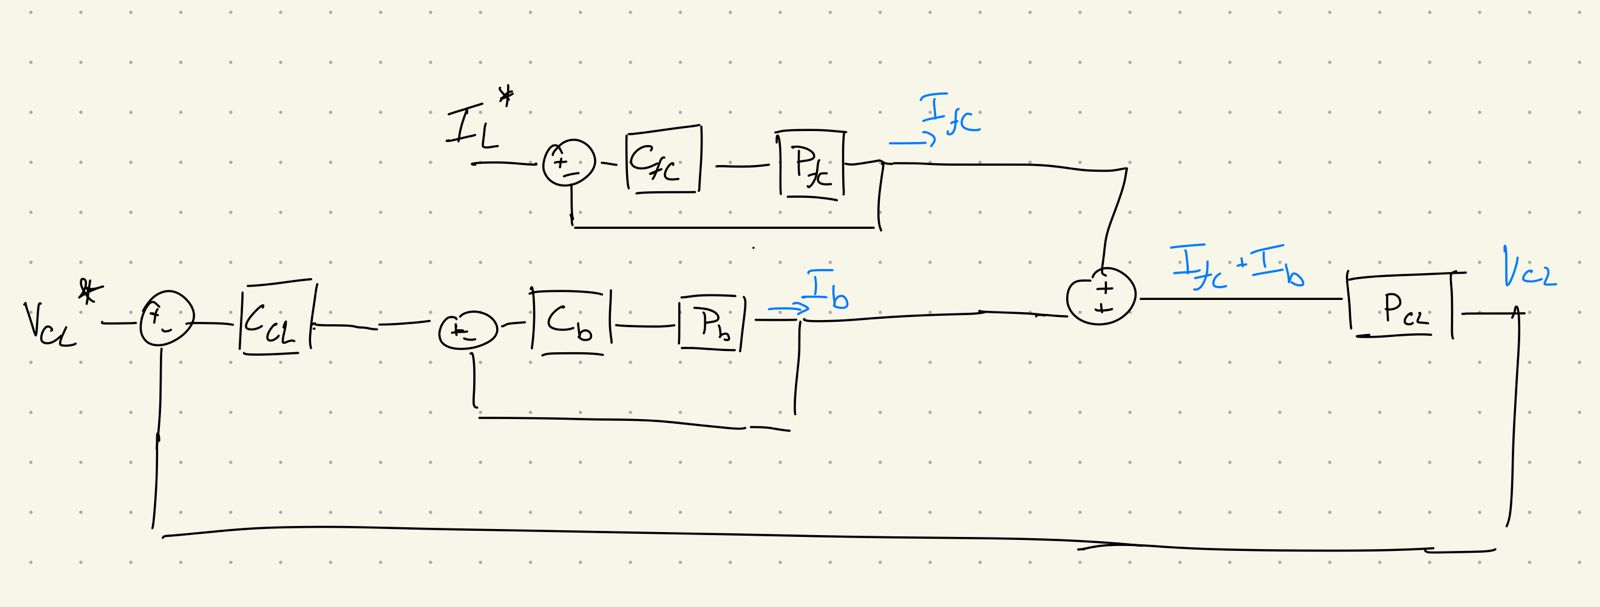
\includegraphics[width=0.7\linewidth]{img/borrador.jpg}
%     \caption{Diagrama de bloques del sistema MIMO}
%     \label{fig:enter-label}
% \end{figure}
Como el sistema se modela con tres funciones de transferencia, entonces son necesarios tres controladores, dos para regular los voltaje de entrada $V_{fc}$ y $V_{B}$ a sus respectivas plantas y uno para regular la corriente en la carga $I_L$. A priori el diagrama de bloques del sistema debería ser de la siguiente forma  
\begin{figure}[htbp]
    \centering
    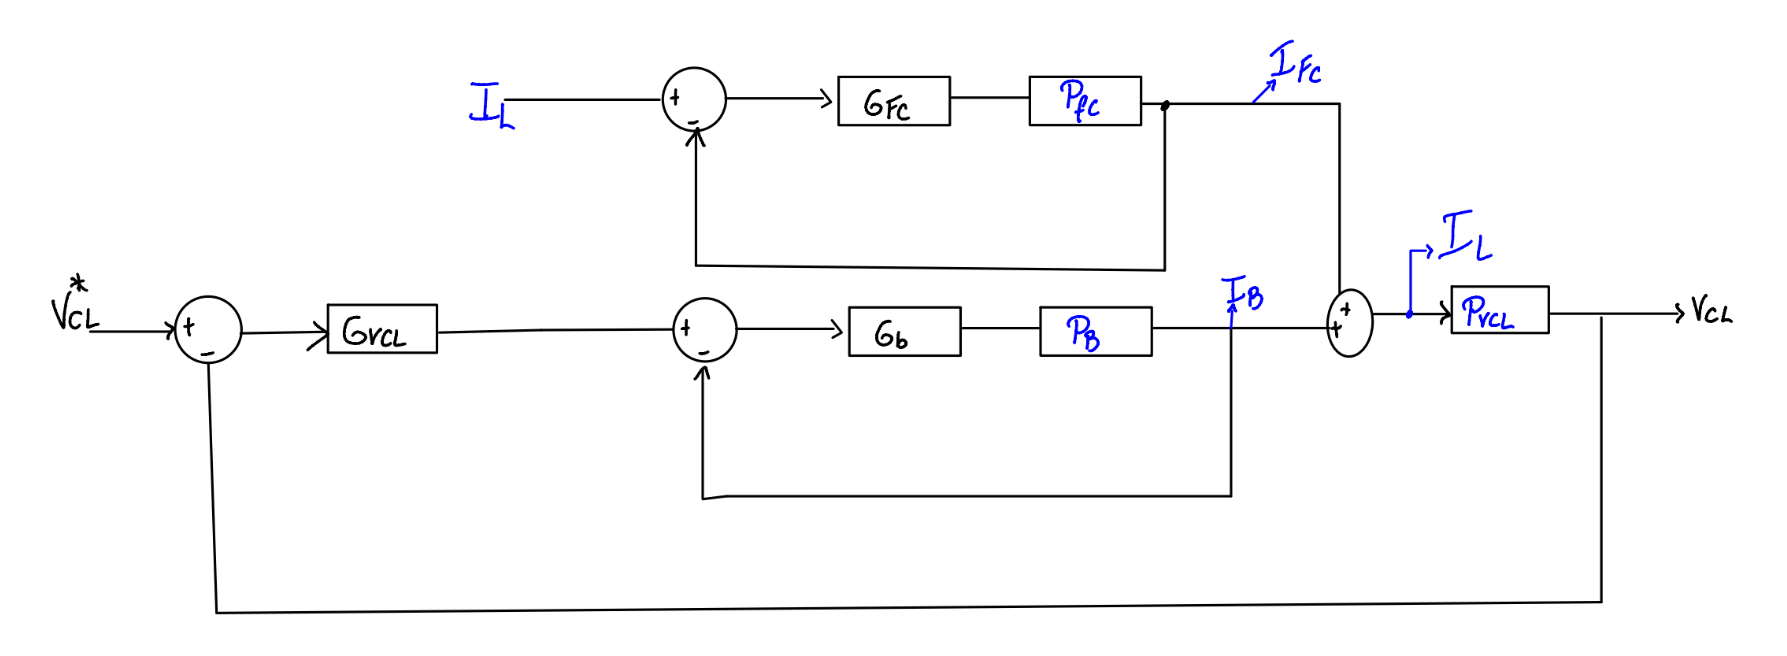
\includegraphics[width=0.9\linewidth]{img/Diagrama de bloques 1.png}
    \caption{Primera iteración diagrama de bloques}
    \label{fig:Diagrama de bloques 1}
\end{figure}

Donde el diagrama de la figura (\ref{fig:Diagrama de bloques 1}) trabaja el control de las corrientes $I_{FC}$ e $I_B$ por separado para luego sumarlas y entregar un valor de $I_L$ que de acuerdo a la naturaleza de la planta entregaría el valor esperado de $V_{CL}$. Ademas, este modelo garantiza que la corriente entregada por la batería tienda a 0 en estado estacionario, pues la referencia del lazo de control de la fuel cell es justamente la corriente de carga $I_L$, por ende en estado estacionario $I_{FC}$ tiende a $I_L$. 

El diagrama de la figura (\ref{fig:Diagrama de bloques 1}) entrega un buen primer acercamiento para el modelamiento del sistema, pero aun está incompleto, pues no explica de donde obtener la referencia de $I_L$ presente en el lazo de la fuel cell, ademas, tampoco considera las limitaciones fisicas de los componentes y por ultimo no se esquematiza el termino $-V_{CL}$ presente en la entrada de las funciones de transferencia (\ref{Funcion de transferencia fuel cell}) y (\ref{Funcion de transferencia batería interno}).

Para complementar el diseño, primero notar que es posible obtener una referencia de $I_L$ a partir de la salida del sistema $V_{CL}$, solo es necesario seguir la ley de ohm y divdir por el valor de la impedancia en la carga, donde no es necesario considerar la capacitancia $C_L$, pues esta tenderá a 0 en estado estacionario pues la batería entrega corriente continua la cual saturará al capacitor. Esta nueva modificación se presenta en la figura (\ref{fig:Diagrama de bloques 2}).

\begin{figure}[htbp]
    \centering
    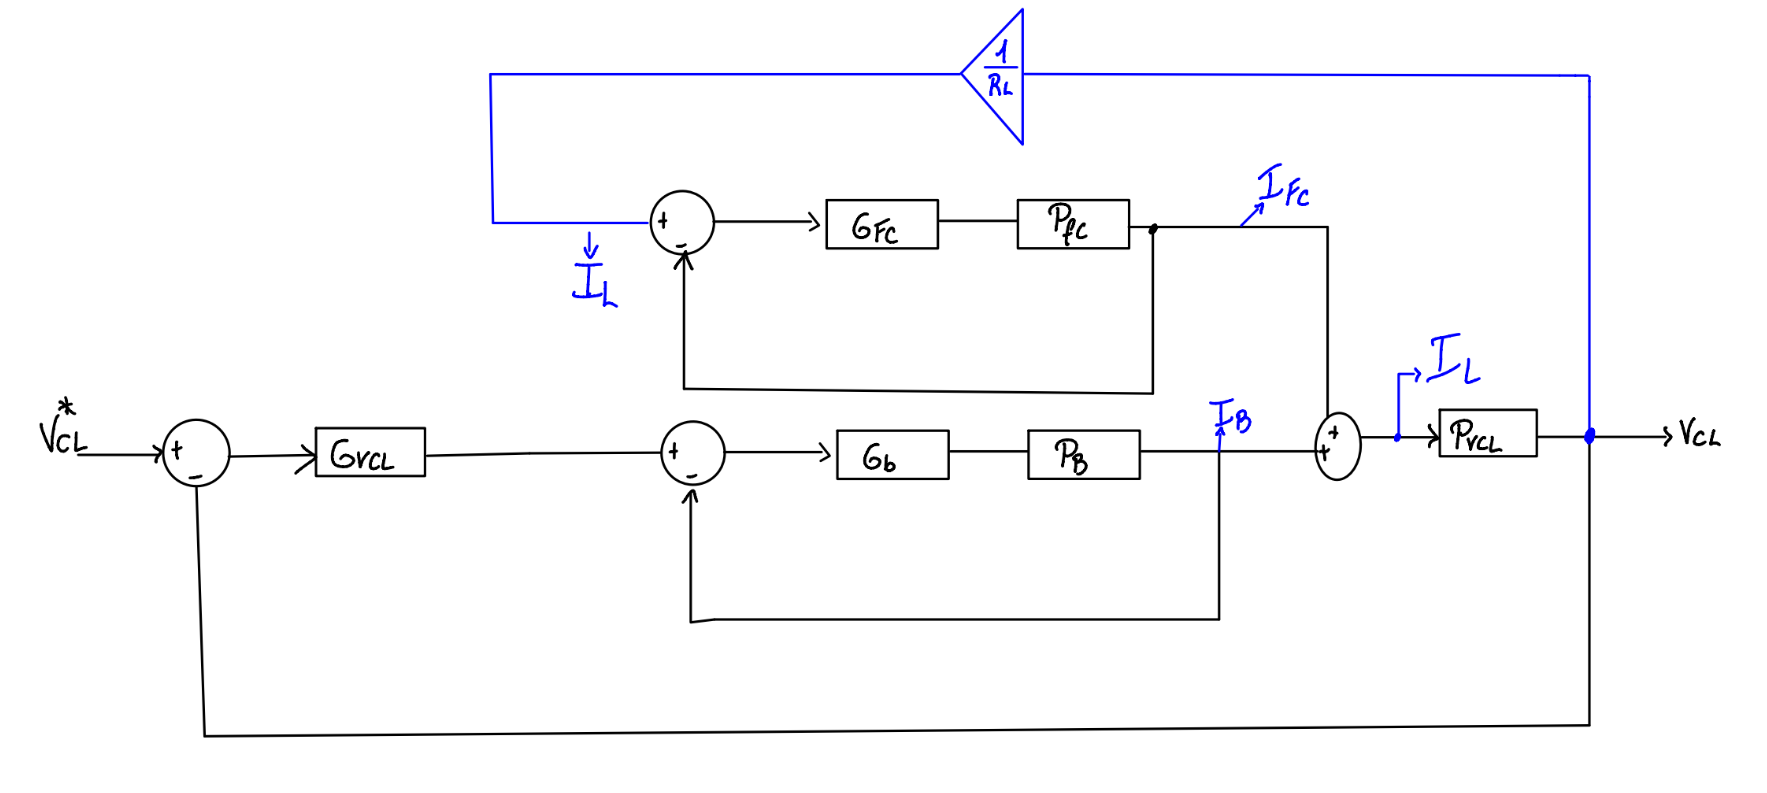
\includegraphics[width=\linewidth]{img/Diagrama de bloques 2.png}
    \caption{Segunda iteración con referencia $I_L$}
    \label{fig:Diagrama de bloques 2}
\end{figure}

Luego, es necesario agregar las limitantes físicas de los componentes del sistema, en la figura (\ref{fig:Diagrama de bloques 3}) se visualizan los ajustes realizados, donde se agregaron los valores limites para $V_{FC}$, $V_{B}$, $I_{FC}$ e $I_{B}$. Finalmente en la figura (\ref{fig:Diagrama de bloques 4}) se agrega el termino faltante $-V_{CL}$.
\newpage

% \begin{figure}[htbp]
%     \centering
%     \begin{subfigure}[b]{0.7\linewidth}
%         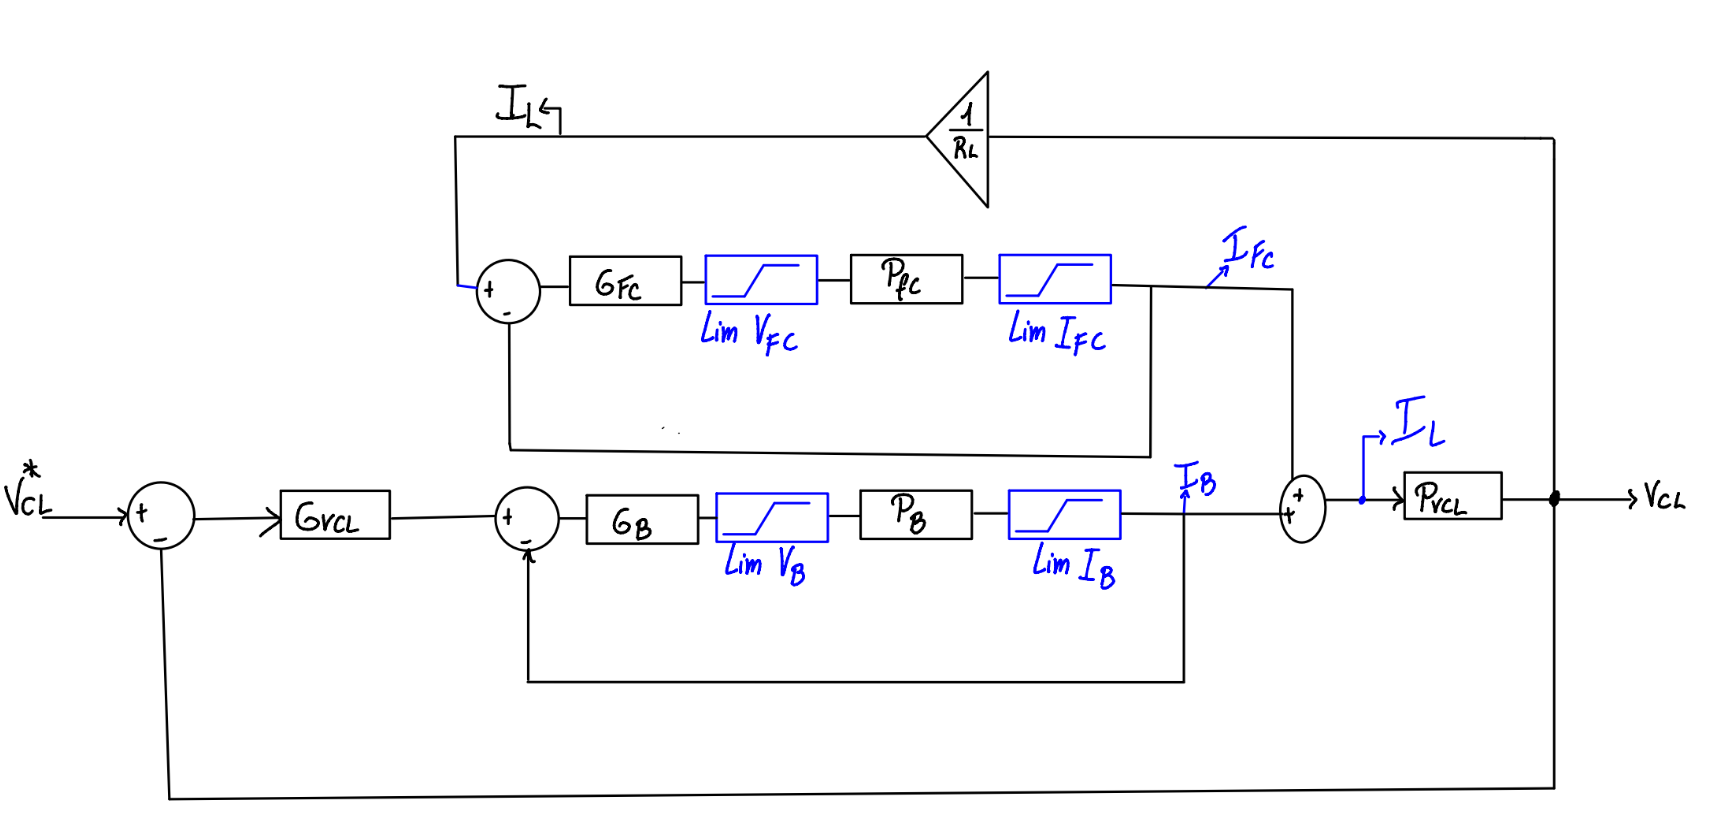
\includegraphics[width=\linewidth]{img/Diagrama de bloques 3.png}
%         \caption{Diagrama de bloques con limitadores}
%         \label{fig:Diagrama de bloques 3}
%     \end{subfigure}
%     \hfill
%     \begin{subfigure}[b]{0.7\linewidth}
%         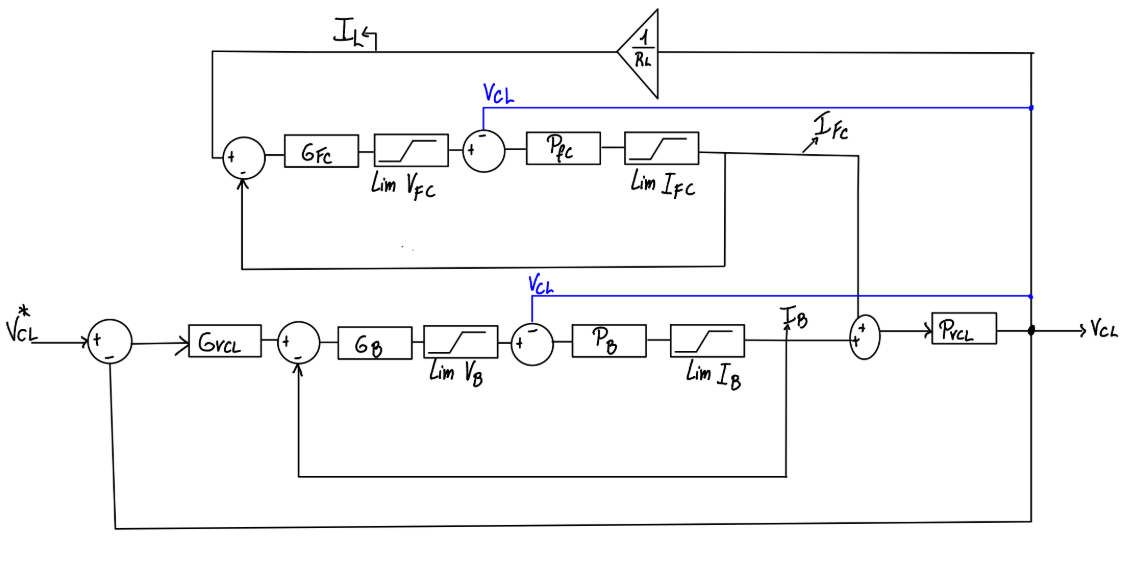
\includegraphics[width=\linewidth]{img/Diagrama de bloques 4 final.png}
%         \caption{Diagrama de bloques con termino faltante $-V_{CL}$}
%         \label{fig:Diagrama de bloques 4}
%     \end{subfigure}
% \end{figure}

\begin{figure}[htbp]
    \centering
    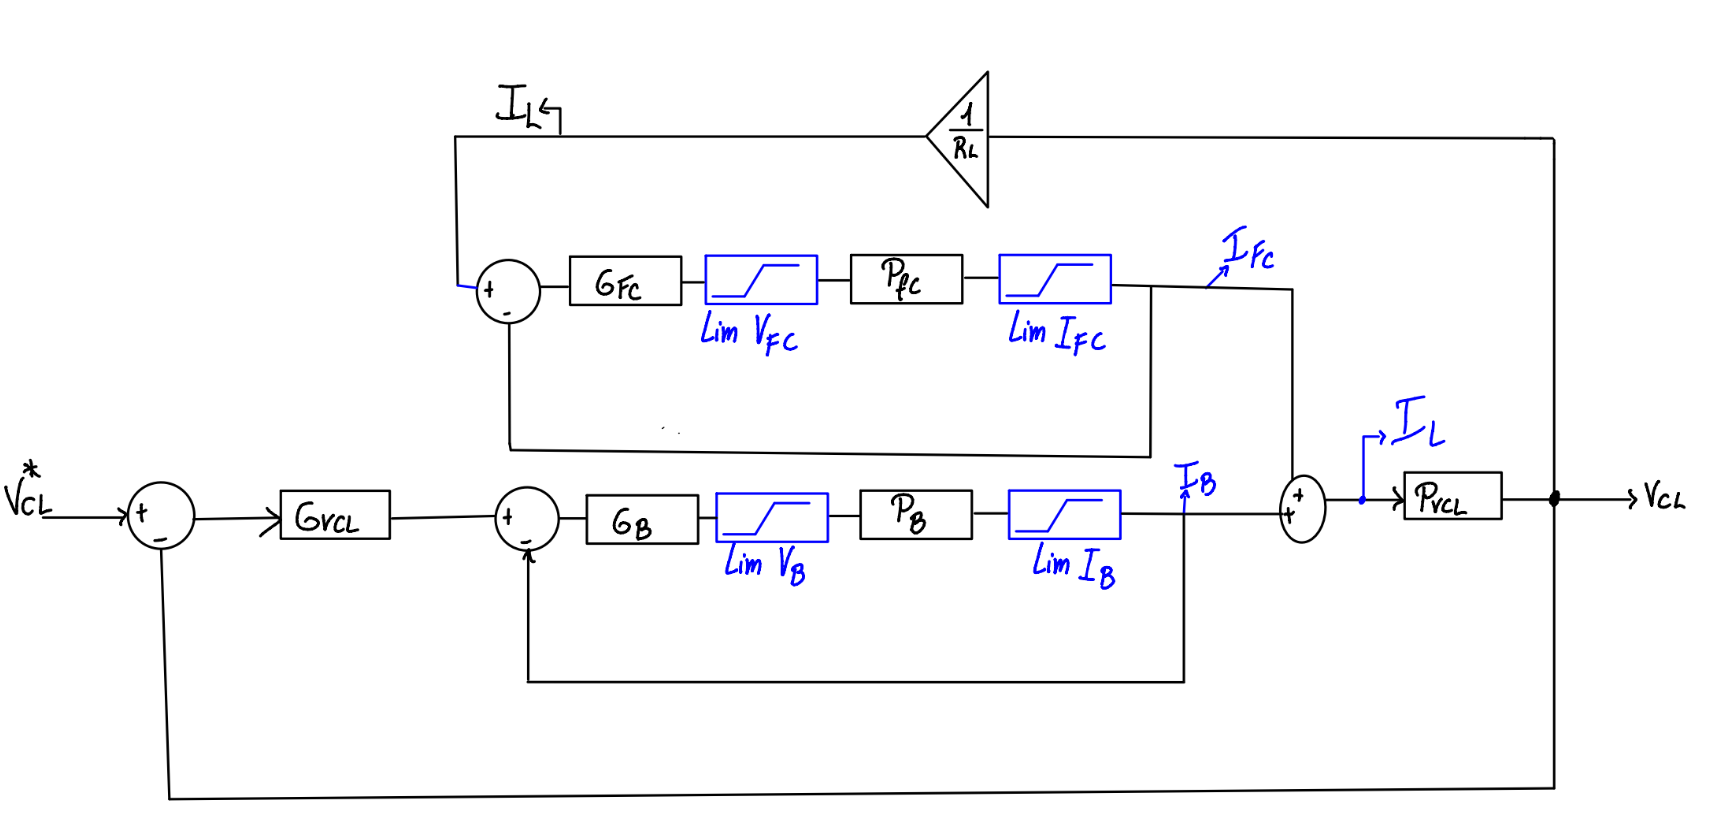
\includegraphics[width=0.85\linewidth]{img/Diagrama de bloques 3.png}
    \caption{Diagrama de bloques con limitadores}
    \label{fig:Diagrama de bloques 3}
\end{figure}
\begin{figure}[htbp]
    \centering
    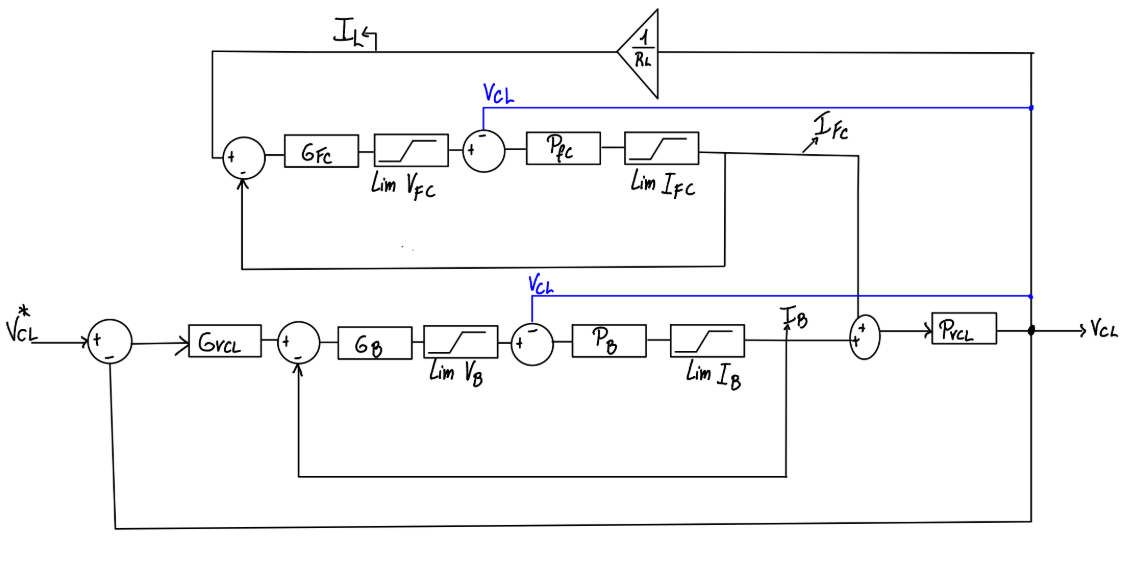
\includegraphics[width=0.85\linewidth]{img/Diagrama de bloques 4 final.png}
    \caption{Diagrama de bloques con termino faltante $-V_{CL}$}
    \label{fig:Diagrama de bloques 4}
\end{figure}

Por ultimo al evaluar los valores respectivos en las ecuaciones (\ref{Funcion de transferencia batería interno}), (\ref{Funcion de transferencia fuel cell}), (\ref{Funcion de transferencia batería externo}) se obtiene la forma de las plantas, las cuales son:


\begin{equation}
    P^B_{int} = \frac{1}{0.003s+0.3}
\end{equation}
\begin{equation}
    P^B_{ext} = \frac{10}{0.04s+1}
\end{equation}
\begin{equation}
    P_{FC} = \frac{1}{2s+0.7}
\end{equation}

\newpage

\subsection{\textit{LGRs y Controladores}}
Una vez ya definidas las plantas del sistema, entonces se procedió a diseñar los respectivos controladores. Se siguió la estructura de controladores tipo PI entonces gracias a la herramienta rtool de MATLAB los controladores para el lazo interno y externo de las baterías son,

\begin{equation}
    G^B_{int} = 6.415\cdot \frac{s+916}{s} \;\text{| } w_{n} = 1400\;  rad/s, \;\zeta = 0.8
\end{equation}
\begin{equation}
    G^B_{ext} = 0.7961\cdot \frac{s+98.5}{s} \;\text{| } w_{n} = 140\;  rad/s, \;\zeta = 0.8
\end{equation}
Ademas se presentan los LGRs obtenidos al momento de realizar el diseño.
\begin{figure}[htbp]
    \centering
    \begin{subfigure}[b]{0.48\linewidth}
        \includegraphics[width=\linewidth]{img/LGRs/LGR batería externo.png}
        \caption{LGR batería externo}
        \label{fig:externa}
    \end{subfigure}
    \hfill
    \begin{subfigure}[b]{0.48\linewidth}
        \includegraphics[width=\linewidth]{img/LGRs/LGR Batería interno.png}
        \caption{LGR batería interno}
        \label{fig:interna}    
    \end{subfigure}
    
\end{figure}

De manera análoga para el control de fuel cell se diseñó un PI de la forma,
\begin{equation}
    G_{FC} = 13.69\cdot \frac{s+2.33}{s} \;\text{| } w_{n} = 4\; rad/s, \;\zeta = 0.9
\end{equation}

Y su LGR respectivo se representa en la figura (\ref{fig:LGR fuel cell})
\begin{figure}[H]
    \centering
    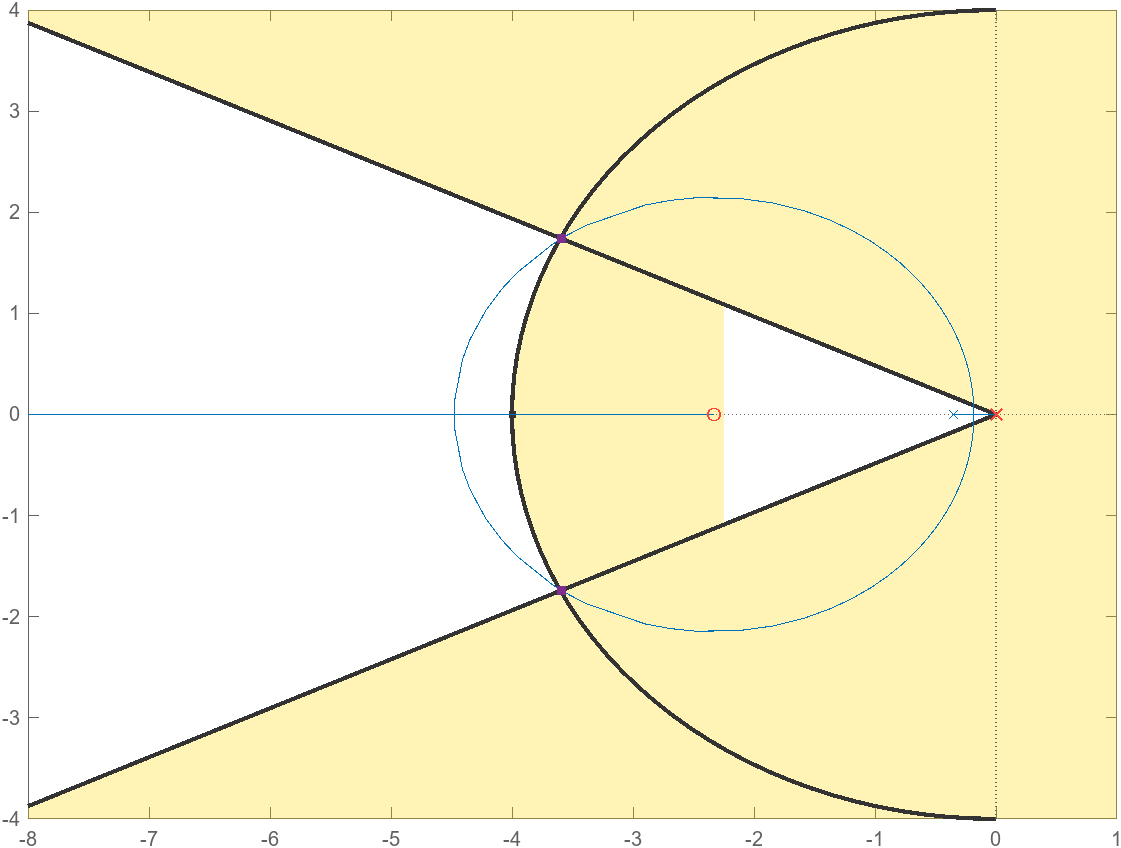
\includegraphics[width=0.5\linewidth]{img/LGRs/LGR fuel cell.png}
    \caption{LGR fuel cell}
    \label{fig:LGR fuel cell}
\end{figure}
% AYUDAAAAAAAAAAAAAAAA VAN A SER LA 1 AM


\newpage